% !TEX root = ../HDR.tex
%%%%%%%%%%%%%%%%%%%%%%%%%%%%%%%%%%%%%%%%%%%%%%%%%%%%%%%%%%%%%%%%%%%%%%%%%%%%%%%%%%
\chapter{Vers une robotique développementale (en construction)}
\label{chap:perspective}

% Cette section pourrait etre incluse dans la précédente "Apprentissage spatio-séquentiel".


Ce chapitre examine comment les mécanismes de schema spatiaux pourraient trouver des applications en robotique. 
Il nous a conduit à mettre en place des euristiques motivationnelles plus complexes 


Deux pistes sont envisagées: les \an{pet robots} et l'augmentation de l'autonomie des drones. 
Les \an{pet robots} ne sont pas vraiment utiles au sens ou ils pourrait réaliser des taches pour les humains, mais il pourraient néammoins trouver des débouchés commerciaux si on en juge par la valeur du marché des animaux de compagnie. 
L'amélioration de l'autonomie des drones pourrait trouver toutes sortes d'usage mais pose des questions éthiques. 


\section{Inférence de structures spatiales}

Introduction en construction

Cette section rapporte des études que nous avons menées pour examiner comment relâcher les présupposés qui sont incorporés dans le modèle SEDP et codés en dur dans ECA. 
Ces études illustrent différentes variantes de l'EDP et différentes formes d'application du principe d'engagement à la causalité.
L'agent est doté de capacités mémorielles qui sous-tendent la construction d'hypothèses d'existence de phénomènes dans l'espace pour expliquer les régularités observées dans le flux d'expérience.

%sous forme du point $\epsilon$ et du déplacement $\iota$, ainsi que Les capacités d'ECA à gérer ces informations par sa mémoire spatiale et son mécanismes de construction de \an{bundles} pourraient reposer sur des principes de plus bas niveau.

%sur des agents modélisés avec l'EDP, afin d'examiner comment ils pourraient découvrir la structure spatiale de leur environnement.  Il s'agit de mieux comprendre comment les structures spatiales codées en dur dans ECA pourraient émerger de principes de plus bas niveau, et de préciser quels seraient ces principes. Leur objectif est d'identifier des principes généraux susceptibles de rendre compte de l'émergence d'une architecture spatiale telle qu'ECA, sans que celle-ci soit codée en dur comme nous l'avons fait pour SEDP, détaillé en Section~\ref{sec:couplage_spatial}. 





\subsection{Espace comme séquence latente et flux optique}
\label{sec:simon}

\noindent
Simon Gay a développé un mécanisme a de représentation de l'espace par séquences latentes d'interactions qui exploite le flux optique  \cite[\an{Autonomous construction and exploitation of a spatial memory by a self-motivated agent}]{gay_autonomous_2017}.
L'expression \emph{espace comme séquence latente} (\an{space as a latent sequence}) est apparue plus tard dans les travaux passés en revue en Section~\ref{sec:structure_spatiale}.  

Ce travail se base sur un modèle EDP dans lequel l'agent reçoit une ensemble d'événements d'interaction à chaque cycle. 
Cet ensemble contient une interaction composée d'un tuple \interaction{decision, outcome} similaires à celles des expérimentations précédentes, à laquelle s'ajoutent des événements de flux optique liés aux points saillant du champ visuel.
Chaque événement de flux optique prend la forme d'un tuple $(c, \theta, v)$ dans lequel $c$ représente la couleur du point saillant, $\theta \in [-\pi/2, \pi/2]$ son angle de coordonnée polaire dans le champ visuel, et $v$ sa vitesse angulaire instantanée polaire. 
%L'agent ne perçoit pas la distance des points saillants.

L'agent dispose de cinq décisions: \texttt{move forward}, \texttt{turn left 90}, \texttt{turn right 90}, \texttt{turn left 45},  \texttt{turn right 45}. 
La décision \texttt{move forward} peut générer les \an{outcome} \texttt{empty}, \texttt{bump}, ou \texttt{eat}, résultant en des interactions de valences 5, -10 et 50. 
Les interactions de rotation ont toutes la valence -3. 


La Figure~\ref{fig:robot_simon} montre les conditions expérimentales utilisant un robot conçu spécifiquement avec des Lego dans un environnement similaire à l'expérimentation des requins de la Section~\ref{sec:requins}.
Le robot contient un capteur de collision servant à générer l'\an{outcome} \texttt{bump}, un capteur de couleur situé sous lui servant à générer l'\an{outcome} \texttt{eat}, et une caméra servant à générer les événements de flux optique.
L'environnement contient des murs verts, des zones rouges traversables, et de zones bleues représentant des cibles qui affordent l'interaction \interaction{move forward, eat}.
Lorsque le robot atteint une cible, l'expérimentateur la retire et en introduit une nouvelle à un autre emplacement.



\begin{figure}[ht]
	\centering
	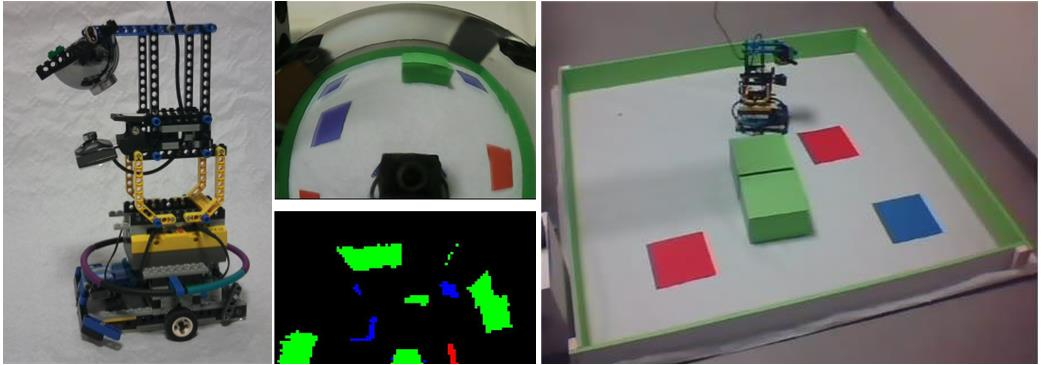
\includegraphics[width=0.9\textwidth]{Figures/3_robot_simon.jpg}
	\caption{%Expérimentation du flux optique \cite[Fig.~4, 5, 8]{gay_autonomous_2014}.
	Gauche: robot disposant d'une caméra orientée vers un miroir sphérique offrant une vision panoramique. 
	Centre: traitement d'image générant des événements de flux optiques.
	Droite: arène répliquant l'expérimentation des requins.}
	\label{fig:robot_simon}
\end{figure}


La figure~\ref{fig:simon_spatial} illustre de manière schématique la façon dont l'agent représente sa situation (gauche) par un ensemble de séquences (centre).
% issue d'une expérimentation des requins similaire à celle décrite en Section~\ref{sec:requins}. 
La partie droite montre une reconstitution de l'espace à destination du lecteur qui n'est pas explicitement réalisée par l'agent lui-même.
Dans cet exemple, les décisions \texttt{turn} peuvent donner lieu à des \an{outcome} \texttt{bump} quand l'agent se tourne vers un mur.
Les séquences se décomposent en deux parties: une partie \emph{chemin} pour atteindre un objet et une interaction finale avec l'objet. 
Lorsque l'agent se déplace, sa représentation de l'espace est mise à jour en fonction des séquences construites lors des interactions précédentes et des événements de flux optique.


\begin{figure}[ht]
	\centering
	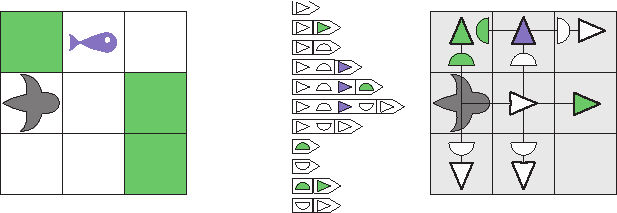
\includegraphics[width=0.7\textwidth]{Figures/3_simon_spatial.pdf}
	\caption{Représentation de l'espace par des séquences latentes d'interactions \cite[Fig~7.2]{gay_mecanismes_2014}.
	Gauche: agent représenté par un requin entouré de murs et d'un poisson.
	Centre: ensemble de séquences affordées par la situation. 
	Droite: reconstitution spatiale à destination du lecteur.
	}
	\label{fig:simon_spatial}
\end{figure}

La correspondance entre les événements de flux optique et les interactions primitives se fait par un mécanisme de \emph{signatures d'interaction}.
La signature d'une interaction primitive permet de calculer la probabilité de pouvoir l'énacter avec succès dans le contexte d'un ensemble d'événements de flux optiques donné. 
L'apprentissage des signatures d'interaction se fait en environnement simulé et demande environ 3000 cycles d'interaction. 
Une fois apprises, elles sont utilisées par le robot pour générer des comportements d'évitement des obstacle et de chasse de cibles. 

Comme ECA, l'architecture de Simon Gay apprend à catégoriser les objets présents dans l'environnement par les \an{bundles} d'interaction qu'ils affordent.
Elle diffère cependant par le fait qu'elle fonctionne sans recevoir la position des objets ni les déplacements du robot (les $\epsilon$ et $\iota$ du modèle SEDP).
Elle est capable d'apprendre en parallèle un modèle de l'espace en termes de séquences latentes, et un modèle des objets en termes de \an{bundles}.
Le modèle spatial permet à l'agent de disposer d'une représentation de sa situation même en dehors de son champ visuel. 

Cette expérimentation illustre comment utiliser la théorie des événements d'interaction valués dans un cadre robotique basé sur le modèle EDP. 
Elle montre comment l'agent peut recevoir une structure de données complexe représentant de nombreux événements d'interaction.  
A notre connaissance, c'est la seule expérimentation démontrent l'acquisition d'une structure spatiale basée sur des séquences latentes qui aie été démontré dans un robot. 
Elle fonctionne par principe en monde ouvert.
La complexité potentiellement infinie du monde est limitée par le fait maitrisée par le fait que l'agent apprend à organiser ses comportements dans le contexte de son champ visuel par nature fini. 
Elle présente toutefois la limitation de nécessiter que l'environnement soit statique. 


Pour des applications nécessitant un apprentissage plus rapide dans un environnement dynamique, elle nous incite à implémenter une carte spatiale explicite et un système de perception des déplacements de l'agent. 

%Tout comme le POMDP permet de modéliser un agent qui reçoit une observation complexe de l'environnement.


\subsection{Construction autonome d'un modèle causal spatial}

\noindent
Un travail exploratoire a été réalisé par Jianyong Xue \cite[\an{Causality reconstruction by an autonomous agent}]{xue_causality_2019}.
L'agent était placé dans un environnement susceptible de présenter un objet à sa droite et un autre à sa gauche. 
Il était doté d'une mémoire spatiale rudimentaire contenant deux emplacements, chacun pouvant prendre trois valeurs distinctes.  
Le but de cette expérimentation était d'étudier les mécanismes nécessaires pour permettre à l'agent d'apprendre à exploiter cette mémoire pour construire une représentation explicite de l'état de l'environnement sur la base des régularités observées dans son flux d'interaction. 

Inspiré de l'expérimentation du \an{Small Loop Challenge}, l'agent disposait de cinq décisions \texttt{feel right}, et \texttt{feel left} pour toucher à droite et à gauche, \texttt{change right} et \texttt{change left} pour supprimer ou faire apparaitre un objet. 
La décision \texttt{feel front} permettait de toucher simultanément à droite et à gauche et renvoyait un outcome lié au nombre d'objets touchés:  0, 1 ou 2.
Comme dans les expérimentations précédentes, l'agent ignorait la signification de ces décisions et \an{outcomes}.
Les valences de toutes les interactions étaient à zéro.

Xue a mis en place une motivation reposant sur une heuristique de recherche de fiabilité rappelant celle implémentée par Drescher (Sec.~\ref{sec:drescher}), couplée à une heuristique d'ennui.
L'heuristique de recherche de fiabilité poussait l'agent à répéter des décisions qui entrainaient toujours les mêmes interactions primitives, jusqu'à ce que l'heuristique d'ennui le pousse à changer de décision. 
Lorsqu'il trouvait une interaction répétable, il l'associait à une valeur prise par un emplacement de sa mémoire spatiale, implémentant ainsi l'hypothèse que cette interaction était affordée par un objet présent dans l'environnement, et que cette valeur pouvait représenter cet objet.
L'agent construisait un graphe de connaissance dont les n\oe uds correspondait à des états uniques de la mémoire spatiale. 
Il construisait ensuite les arcs de ce graphe en leur associant les interactions permettant les transitions d'état correspondants. 
Il utilisait ensuite ce graphe comme un réseau de Petri dans lequel la sitaution courante était marquée par un jeton placé sur un n\oe ud.
L'expérimentation a montré qu'au bout de 350 cycles d'interaction l'agent a pu construire un graphe complet pour représenter la dynamique de son complage avec l'environnement. 
La Figure Figure~\ref{fig:causal}  en donne une représentation partielle. 


\begin{figure}[ht]
	\centering
	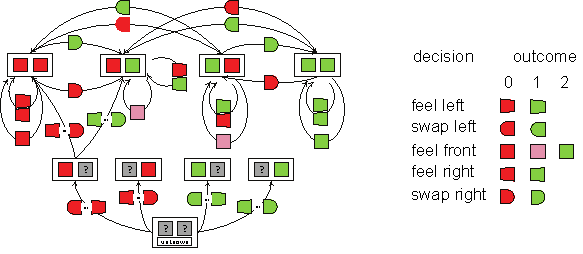
\includegraphics[width=0.6\textwidth]{Figures/3_causal.pdf}
	\caption{Réseau de Petri représentant la structure causale construite par l'agent pour expliquer la dynamique de ses interactions \cite[Fig.~3]{xue_causality_2019}.
		Rectangles blancs: n\oe uds du réseau représentant des états de l'environnement.
		Arcs: transitions d'état associées à des interactions.}
	\label{fig:causal}
\end{figure}

Ce résultat montre que l'agent a pu apprendre à utiliser les deux emplacements de sa mémoire spatiale pour représenter sa connaissance ou non des états possibles de son environnement. 
Il utilisait un des emplacements pour représenter sa gauche, l'autre sa droite. 
Un des états pour représenter qu'il ignorait l'état de l'environnement correspondant, un autre état pour représenter la connaissance de la présence d'un mur, et le troisième la connaissance d'un vide. 
Le graphe obtenue est une sorte de graphe d'habitudes au même titre que celui de Woolford en Figure~\ref{fig:ssr}.


Cette expérimentation suggère que même dans une configuration rudimentaire, l'apprentissage de l'usage d'une mémoire spatiale requiert l'implémentation de présupposés substantiels dans l'agent: des heuristiques comportementales, des traitements spécifiques pour implémenter une hypothèse de causalité, et une structure mémorielle dont la capacité soit adaptée à la complexité des situations rencontrées.
La question de la généralisation de ces principes à des environnements plus riches et à des architectures de mémoire plus complexes demeure ouverte. 



\section{Le projet Petitcat}


\noindent
Ce projet adopte une approche d'ingénierie pragmatique pour étudier comment la théorie des Evénements d'Interaction Valués s'applique à la conception de robots autonomes. 
L'objectif est de générer des comportements jugés naturels et intéressants par un observateur humain. 
Cette approche pragmatique apporte une source d'inspiration pour faire évoluer l'architecture cognitive ECA, dans une logique de rétro-engineering de la cognition.
Par exemple, elle nous a amenés à associer des variables libres aux décisions et aux interactions, rejoignant ainsi des choix de conception pris par d'autres architectures cognitives constructivistes examinées en Section~\ref{sec:architectures}.


L'objectif de génération de comportements en milieu ouvert et dynamique nous conduit à présupposer l'existence d'informations de position des événements d'interaction et de déplacement du robot comme nous l'avons formalisé dans le modèle SEDP. 
Nous avons donc recherché un robot offrant une bonne mobilité, des capteurs capables de renvoyer des informations de position, et dotés d'une unité de mesure inertielle pour fournir certaines informations de déplacement.

Plusieurs plateformes robotiques ont été considérées. 
Outre les robots e-puck et Eddie présentés en Section \ref{sec:sequentiel-robotique}, et la plateforme Lego de la section précédente, nous avons aussi testé la plateforme TurtleBot. 
Le TurtleBot est une plateforme commerciale assez répandue dans les laboratoires de recherche.  
Pour moins de 3000 euros elle embarque un Rasbery Pi hébergeant le logiciel de contrôle robotique ROS, ainsi que des capteurs intéressants tels qu'un lidar et une camera, et une unité de mesure inertielle. 
Ces capteurs la rendent souvent utilisée pour tester des algorithmes de \an{Simultaneaous Localisation and Mapping}. 
A l'usage, cependant, la plateforme ROS s'est montrée inutilement compliquée pour mettre en \oe uvre le modèle SEDP. 
La présence d'un PC embarqué s'est avérée également inutile dans la mesure ou le robot peut être contrôlé à distance via wifi.
% car il est plus pratique d'implémenter ECA sur un PC distant. communiquant avec le robot par wifi.

Nous avons donc opté pour une plateforme contrôlé par une simple carte Arduino, et offrant une meilleure capacité de mobilité que le TurtleBot, la possibilité de capteurs satisfaisant pour l'approche EIV à un moindre coût. 

L'architecture cognitive ECA est implémenté sur un PC distant. Elle transmets la décision via wifi sous la forme d'une trame de caractère UDP. 
La carte Arduino embarquée se charge d'interpréter la décision et de la mettre en \oe uvre, puis de renvoyer les événements d'interaction au PC via wifi sous la forme d'une trame de caractère UDP. 

\subsection{Configuration matérielle}
\label{sec:petitcat_hardware}

\noindent
Nous avons conçu le robot Petitcat en nous appuyant sur une plateforme développée dans le cadre du \an{open source hardware} et commercialisée sous différentes variantes par plusieurs sociétés. 
Cette plateforme offre plusieurs avantages, à commencer par son prix très modeste inférieur à 200 euros. 
Sa tête mobile lui donne une expressivité par sa capacité à s'orienter vers l'objet sur lequel il porte son attention. 
Ses roues ominidirectionnelles permettent une certaine agilité de déplacement.
Son télémètre à ultrason, bien qu'étant un capteur très grossier, offre l'avantage sur une caméra de donner une indication de distance. 
Il est également équipé d'une barre de cinq capteurs infrarouges à l'avant permettant de détecter des contrastes de luminosité sur le sol. 

La carte Arduinon Mega s'avère plus simple qu'un Rasberry pour implémenter le contrôleur primitif des interactions en C++. 
Elle permet un excellent contrôle du cycle d'exécution à une vitesse fiable de l'ordre de la millisecondes. 
Sa flexibilité permet d'ajouter d'autres capteurs selon les besoins. 
A ce jour nous avons ajouté une unité inertielle, un capteur de couleur dirigé vers le sol sous le robot, ainsi qu'une LED multicolore sur son dos (Figure~\ref{fig:petitcat_hardware}). 
L'unité de mesure inertielle contient un accéléromètre linéaire, un gyromètre et une boussole. 



\begin{figure}[ht]
	\centering
	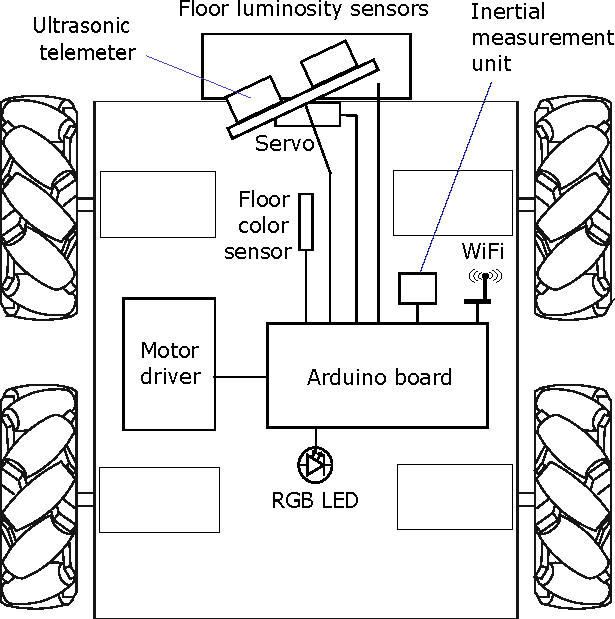
\includegraphics[height=0.35\textwidth]{Figures/4_petitcat_hardware.pdf}%
	\quad
	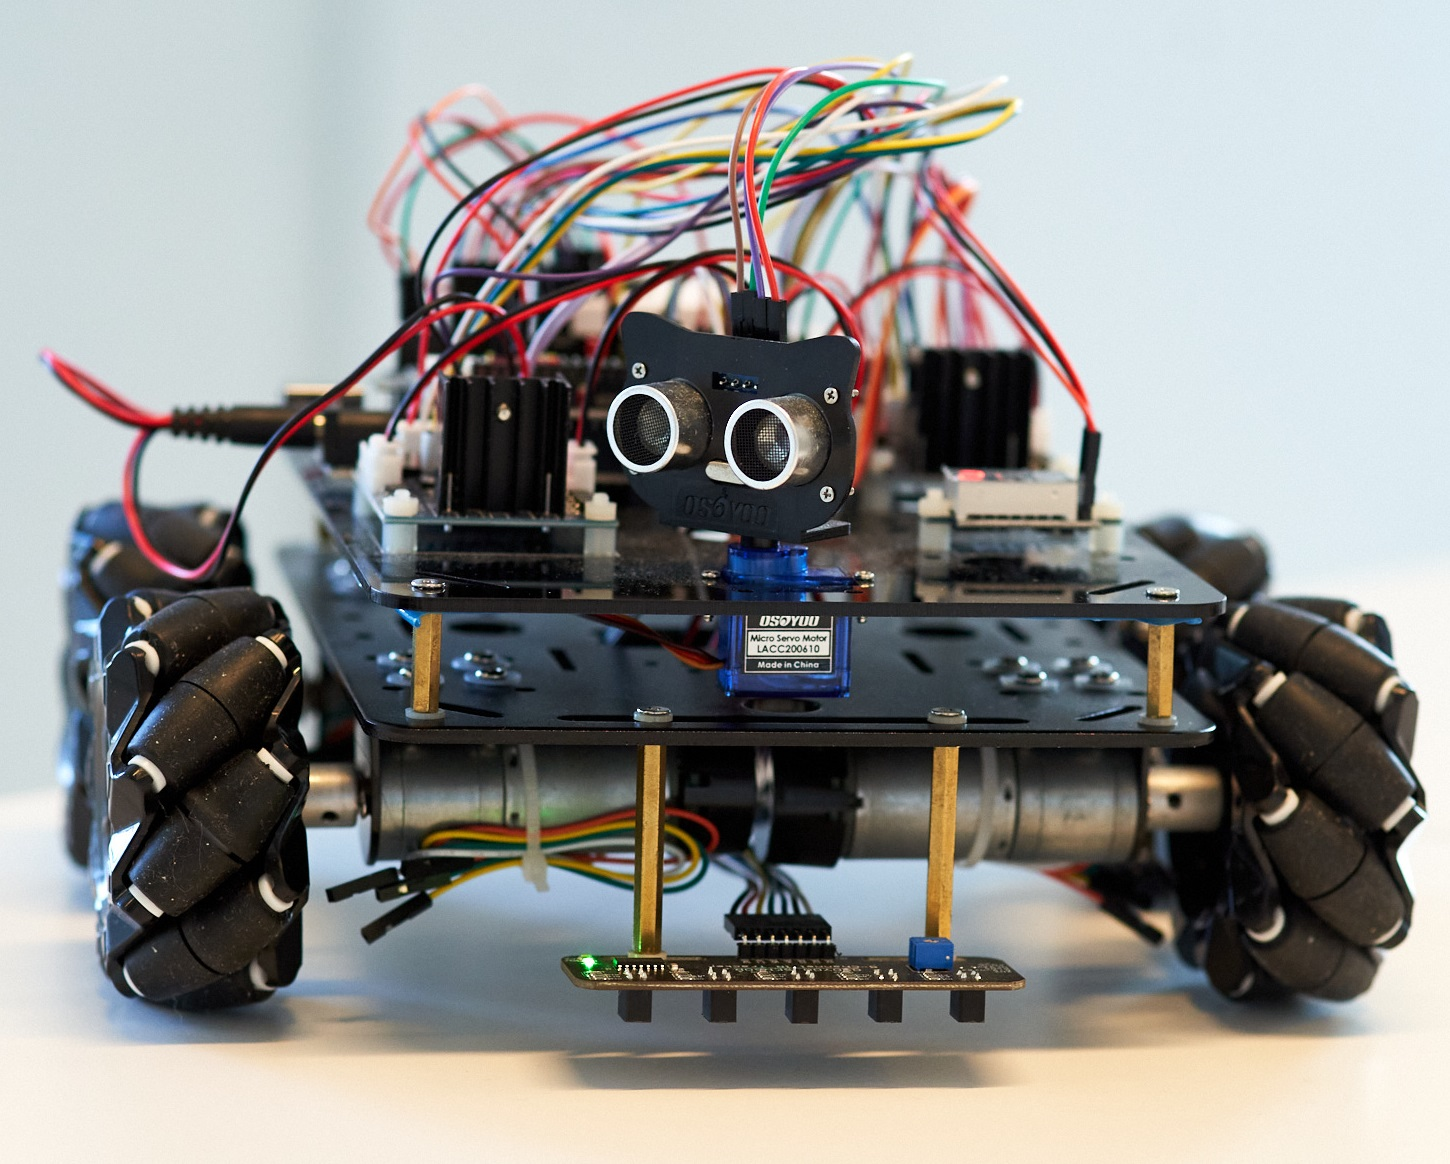
\includegraphics[height=0.35\textwidth]{Figures/4_petitcat_photo.jpg}
	\caption{Robot Petitcat adapté de \cite[Fig.~7 et 8]{georgeon_artificial_2024}.
		Connectée au PC de contrôle via wifi, la carte Arduino pilote l'énaction des décisions en commandant les effecteurs et capteurs: roues omnidirectionnelles, rotation de la tête, télémètre à ultrason, barre de capteurs de luminosité du sol, capteur de couleur du sol, carte inertielle, LED multicolore.
		%, puis renvoie les événements au PC via wifi. 
	} 
	\label{fig:petitcat_hardware}
\end{figure}





\subsection{Possibilités d'interaction}

\noindent
Petitcat implémente le contrôleur primitif chargé de contrôler l'exécution des décisions et de renvoyer les événements d'interaction énactés (Section~\ref{sec:couplage}).
A ce jour il reconnait sept décisions listées dans le Tableau~\ref{tab:decision_petitcat}, qui peuvent être paramétrées par les variables libres du Tableau~\ref{tab:parametres_petitcat}.


Petitcat n'a pas la capacité de mesurer directement sa distance parcourue. 
L'accéléromètre linéaire de la centrale inertielle n'offre pas la précision suffisante pour dériver la vitesse linéaire et encre moins la distance parcourue. 
Les décisions \texttt{move} et \texttt{swipe} peuvent néanmoins être modulées par variable libre spécifiant leur durée: \texttt{duration}. 
ECA peut estimer la distance correspodnante connaissant la vitesse approximative de   $300 mm/s$.

L'angle de rotation associé à la décision \texttt{turn} est spécifié par la variable \texttt{angle} et contrôlé par le gyromètre de la centrale inertielle. 

L'angle de rotation de la tête associé à la décision \texttt{turn-head} est spécifié par la variable \texttt{angle} et exécuté par un servomoteur. 



\begin{table}[h]
	\centering
	\begin{tabular}{|l|l|c|}
		\hline
		\textbf{Code} & \textbf{Description} & \textbf{Paramètre principal}  \\ \hline
		\texttt{move forward} & translation longitudinale vers l'avant & durée (ms) \\ \hline
		\texttt{move backward} & translation longitudinale vers l'arrière& durée (ms) \\ \hline
		\texttt{swipe left} & translation latérale vers la gauche & durée (ms) \\ \hline
		\texttt{swipe right} & translation latérale vers la droite & durée (ms) \\ \hline
		\texttt{turn} & rotation sur place & angle (degrés) \\ \hline
		\texttt{turn-head} & rotation de la tête & angle (degrés)\\ \hline
		\texttt{scan} & série de saccades de la tête & angle (degrés) \\ \hline
	\end{tabular}
	\caption{Décisions primitives reconnues par PetitCat.
	}
	\label{tab:decision_petitcat}
\end{table}

P
Les décisions \texttt{move}, \texttt{swipe}, et \texttt{turn} provoque le déplacement du robot pendant la durée ou l'angle paramétré, mais ces déplacements sont interrompus si une collision est détectée par la centrale inertielle ou si un changement de luminosité est détecté sur le sol.

L'interruption du mouvement en cas de changement de luminosité du sol évite au robot de tomber d'une table ou l'empèche de franchir une ligne noir sur le sol, ce qui permet de le contenir dans une \emph{arène} d'expérimentation. 
La durée écoulée avant cette interuption est renvoyée comme variable de l'interaction énactée. 
Elle permet de calculer une estimation de la distance parcourue. 


 


\begin{table}[h]
	\centering
	\begin{tabular}{|l|l|c|c|}
		\hline
		\textbf{Code} & \textbf{statut}  & \textbf{décision}  & \textbf{Description} \\ \hline
		\texttt{step} & obligatoire & toutes & numéro du cycle d'interaction \\ \hline
		\texttt{decision code} & obligatoire  & toutes & code de la décision \\ \hline
		\texttt{focus-x} & optionnel & \texttt{move}, \texttt{swipe}, \texttt{turn} & coordonnée x du point d'attention \\ \hline
		\texttt{focus-y} & optionnel & \texttt{swipe}, \texttt{swipe}, \texttt{turn} & coordonnée y du point d'attention \\ \hline
		\texttt{color} & optionnel & toutes & couleur de la LED\\ \hline
		\texttt{duration} & optionnel & \texttt{move}, \texttt{swipe} & durée (ms) \\ \hline
		\texttt{angle} & optionnel & \texttt{turn}, \texttt{turn-head}, \texttt{scan} & angle (degrés) \\ \hline
		\texttt{caution} & optionnel & toutes & catégorie de prudence \\ \hline
	\end{tabular}
	\caption{Variables associées aux décisions.
	}
	\label{tab:parametres_petitcat}
\end{table}



\begin{table}[h]
	\centering
	\begin{tabular}{|l|l|}
		\hline
		\textbf{Code} & \textbf{description}   \\ \hline
		\texttt{step} & numéro du cycle d'interaction renvoyé pour vérification \\ \hline
		\texttt{decision code} & décision renvoyée pour vérification  \\ \hline
		\texttt{yaw} & rotation dans le plan horizontal (degrés) \\ \hline
		\texttt{duration} & durée avant interruption (ms) \\ \hline
		\texttt{total duration} & durée totale (ms) \\ \hline
		\texttt{head angle} & direction de la tête \\ \hline
		\texttt{echo distance} & distance mesurée par le télémètre (mm) \\ \hline
		\texttt{floor} & code capteur de luminosité du sol \\ \hline
		\texttt{color} & code capteur de couleur du sol \\ \hline
		\texttt{azimuth} & direction de la boussole  \\ \hline
		\texttt{impact} & code d'impact mesuré par la plateforme inertielle  \\ \hline
		\texttt{echoes} & tableau des distances mesurées pendant l'interaction \texttt{scan}  \\ \hline
	\end{tabular}
	\caption{Variables définissant les événements d'interaction.
	}
	\label{tab:interactions_petitcat}
\end{table}


\subsection{Place cells}

Les \an{schemas mechanisms} offrent la possibilité d'être \og ensemencés \fg avec des comportements prédéfinis. 
Ceci peut être fait dans un esprit d'analogie avec les animaux qui naissent avec de nombreux comportements hérités de leurs ancêtres. 
Il n'est pas forcément nécessaire qu'un robot apprenne de manière autonome des comportements intelligents à partir de zéro pour qu'il exhibe des propriétés comportementale utiles. 
On peut imaginer des robots avec des comportements prédéfinis que s'activent dans des situations variées et qui pourraient exhiber des propriétés intéressantes pour un compagnon humain. 



\begin{figure}[ht]
	\centering
	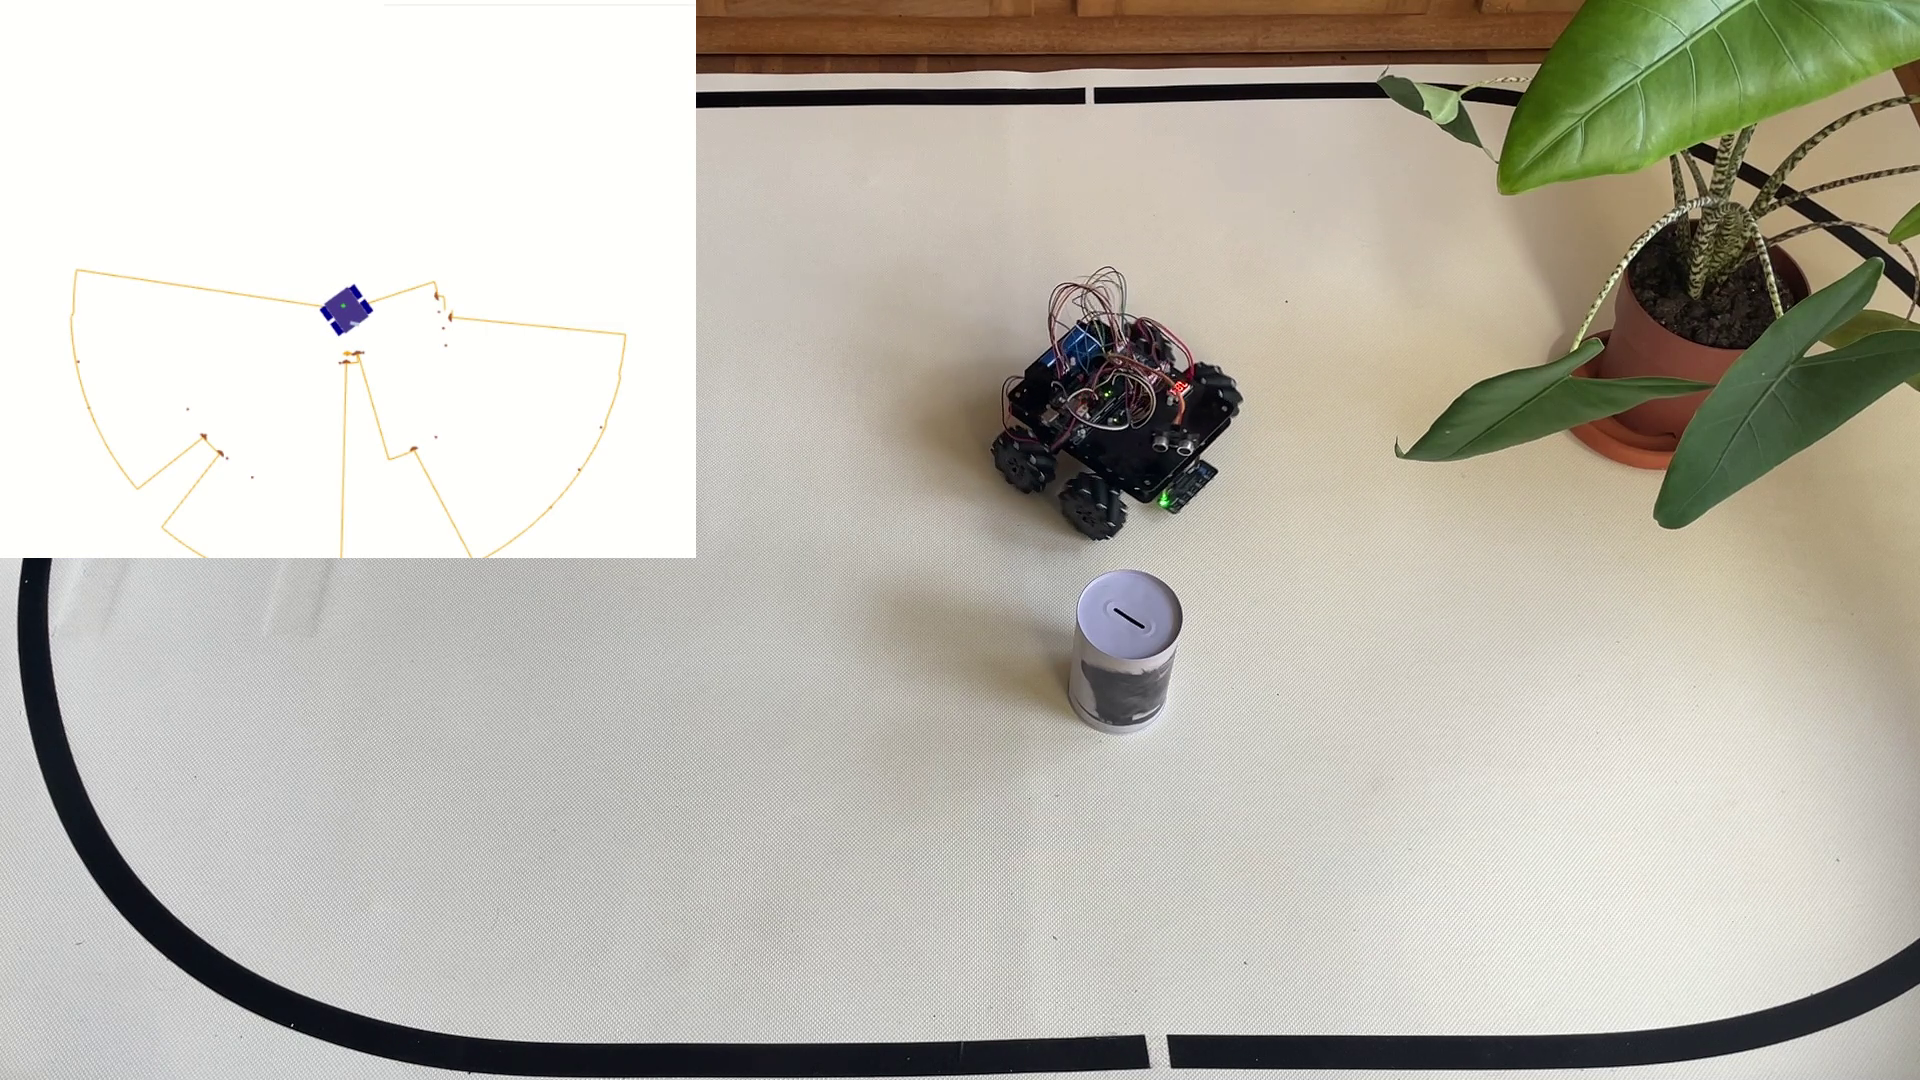
\includegraphics[height=0.3\textwidth]{Figures/4_place_experiment.png}%
	\quad
	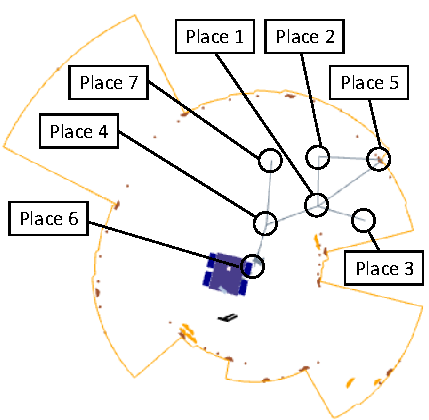
\includegraphics[height=0.3\textwidth]{Figures/4_place_path.pdf}
	\caption{Expérimentation des places \cite[Fig.~1 et 3]{georgeon_spatio-temporal_2026}.
	} 
	\label{fig:place}
\end{figure}


%Le nouveau système perceptif possède une architecture duale qui intègre un \emph{canal perceptif dynamique} et un \emph{canal perceptif statique}.
%Le canal perceptif dynamique est similaire à celui présenté en Section \ref{sec:horseshoe}: il renvoie les \an{outcomes} dynamiques définis en Section \ref{sec:horseshoe} par rapport à la cible sélectionnée par le système motivationnel: apparition, rapprochement, éloignement.  

\subsection{Simultaneous Localisation And Phenomenon Inference}



 \cite[\an{Simultaneous Localisation and Phenomenon Inference}]{georgeon_simultaneous_2022}.


\begin{figure}[htbp]
	\centering
	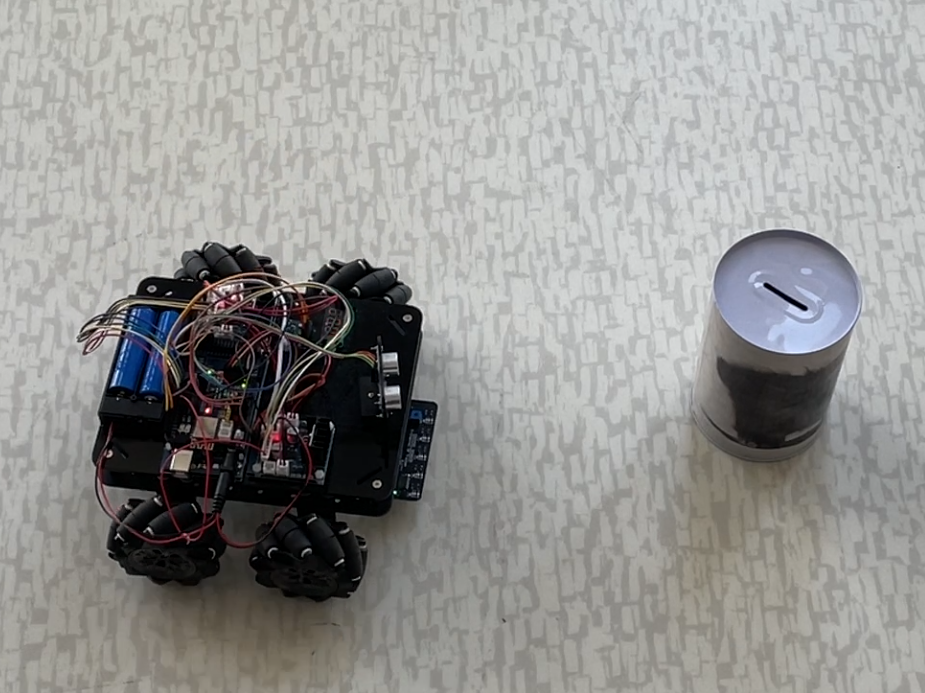
\includegraphics[width=0.49\textwidth]{Figures/6_moneybox.png}
	\hfill
	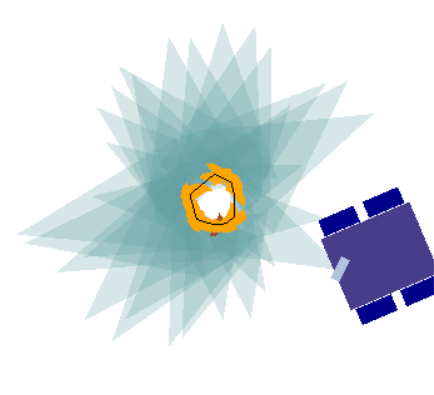
\includegraphics[width=0.49\textwidth, trim = 0 20 0 0, clip]{Figures/6_phenomenon.png}
	\caption{Apprentissage d'un phénomène représentant un objet cylindrique \cite[Fig.~13]{georgeon_schema_2025}.
		Gauche: le robot observant l'objet. 
		Droite: le phénomène identifié par le robot. 
		Le phénomène est constitué de l'ensemble des \og manifestations \fg de l'objet cylindrique à travers les meures d'écho-localisation réalisées quand le robot tourne autour de lui. 
		Les triangles bleus représentent les cônes du signal ultrasonique émis depuis différentes positions. 
		La ligne noire est la forme du phénomène reconstituée à parti des échos.
	}
	\label{fig:robot}
\end{figure}



\subsection{Enseignements}


A partir du moment ou le robot peut activer plusieurs effecteurs en parallèle se pose la question de savoir s'il doit être doté de la capacité de prendre plusieurs décisions en parallèle. 
Nous imaginons qu'une telle éventualité impliquerait l'existence de plusieurs agents EDP qui controleraient le même robot tout en apprenant à se synchroniser entre eux. 
Nous n'avons pas encore exploré cette voie et nous nous limitons pour l'instant à une seule décision par cycle d'interaction, qui peut entrainer plusieurs commandes d'effecteurs contrôlées par les variables libre de la décision.


Elle nous a conduit à examiner des systèmes motivationnels basé sur des états émotionnels et à renoncer pour le moment à une apprentissage des structures spatiales à partir de zéro dans un milieu ouvert. 


Par exemple, Elle nous a conduit à examiner des systèmes motivationnels basé sur des états émotionnels et à renoncer pour le moment à une apprentissage des structures spatiales à partir de zéro dans un milieu ouvert. 
Elle nous a conduit à examiner des systèmes motivationnels basé sur des états émotionnels et à renoncer pour le moment à une apprentissage des structures spatiales à partir de zéro dans un milieu ouvert. 

nous avons été amenés à associer des variables libres aux décisions et aux interactions, rejoignant ainsi des choix de conception pris par d'autres architectures cognitives construcgtivistes examinées en Section~\ref{sec:architectures}.


Nous avons besoin de schémas qui ne capturent pas seulement des séquences d'interactions, mais qui capturent plus généralement des organisation spatio-temporelles d'interactions. 
Pour cela nous conservons la notions de \emph{variable libres} dans les schémas qui peuvent être renseignées au moment de leur tentative d'énaction en fonction de l'état de différents modèles mentaux de l'agent. 



\section{Architecture cognitive}

\begin{figure}[ht]
	\centering
	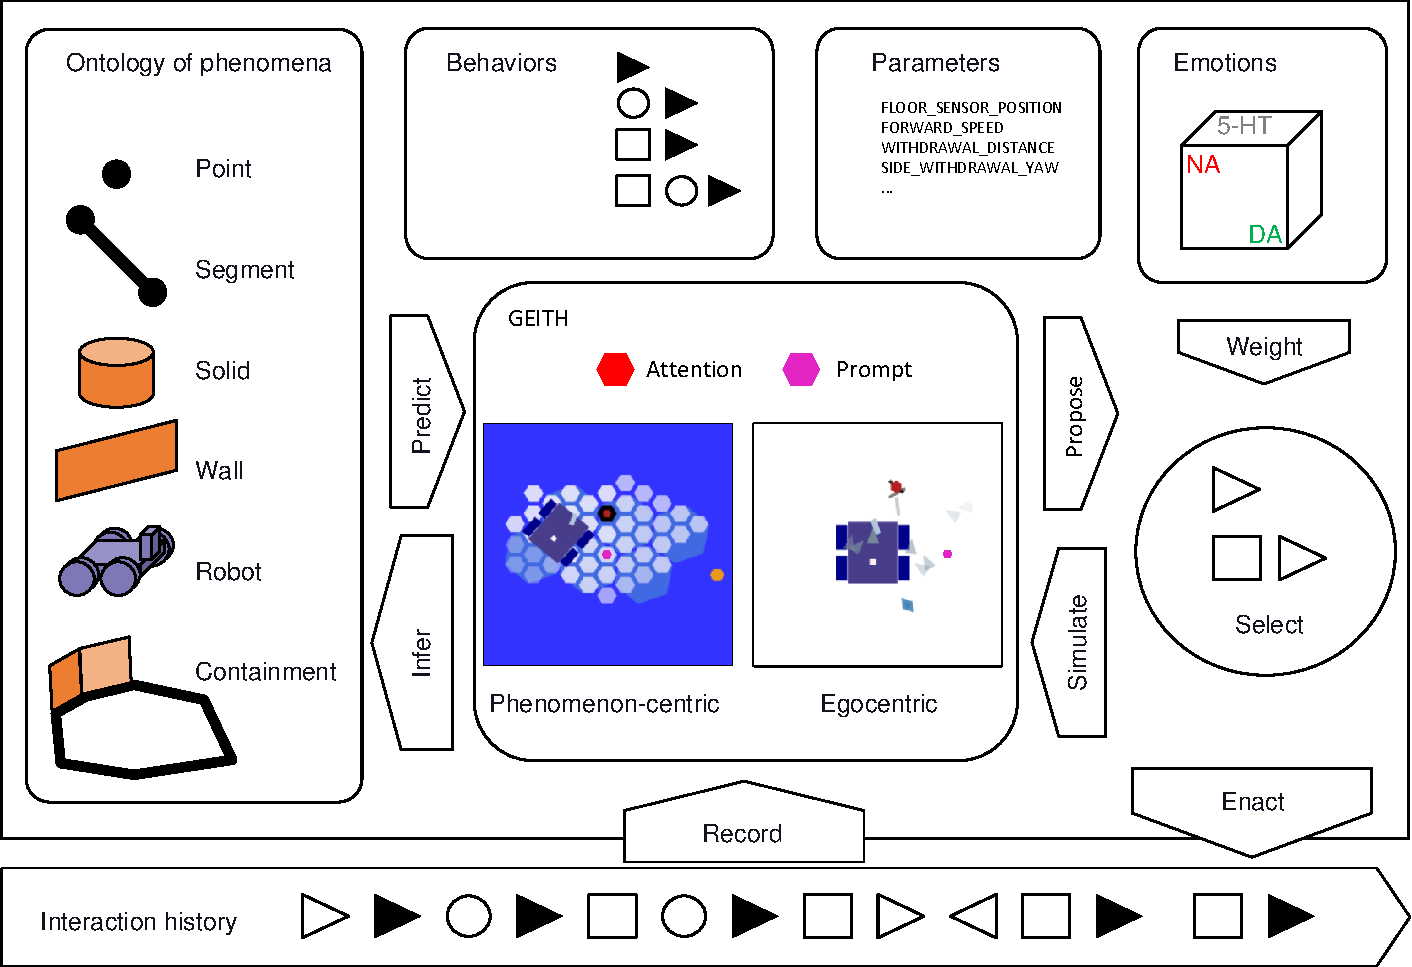
\includegraphics[width=0.6\textwidth]{Figures/4_GEITH.pdf}
	\caption{Architecture cognitive incluant le Game Engine In The Head \cite{georgeon_reducing_2024}}
	\label{fig:GEITH}
\end{figure}


Permet une simulation interne.
Implémente l'idée d'un Game Engine In the HEAD. 

La Figure \ref{fig:petitcat} montre le robot Petitcat.


\section{Conclusion}


La connaissance pourrait etre ancrée dans des schémas acquis par un autre robot. 
Il serait intéressant de savoir quel serait le niveau plus élevé de de grounding qui pourrait etre utilsé par un autre agent. 

Cette approche a été nommée interactionisme radical \cite{georgeon_radical_2013}

Le EDP peut etre simplifié en nommant interaction les couples $\langle action, outcome \rangle$.
Une interaction peut etre utilisé comme un élément fondamental du modèle qui represente un scheme sensorimoteur piagetien $ i = \langle a, o \rangle $. 

\cite{georgeon_radical_2013}

L'interactionisme radical est illustrée en Figure \ref{fig:ir}.
A chaque temps de décision $d$, l'agent sélectionne une interaction composite $i_{cd}$ appartenant à l'ensemble $C_d$ des interactions composites connues au temps $d$.
Enacter $i_{cd}$ consiste à successivement tenter d'enacter les $j$ interactions primitives $i_{p1}$ à $i_{pk}$. 
Si chaque chaque interaction primitive est enactée avec succès ($e_{pj} = i_{pj}, j \in [1...k]$), alors l'agent reçoit l'interaction composite $e_{cd} = i_{cd}$.
Si l'enaction d'une interaction $i_{pj}$ échoue alors l'énaction de $i_{cd}$ échoue et $e_{cd}$ est construite à partir de la série $\langle e_{p1}, ..., e_{pj} \rangle$.

\begin{figure}[ht]
	\centering
	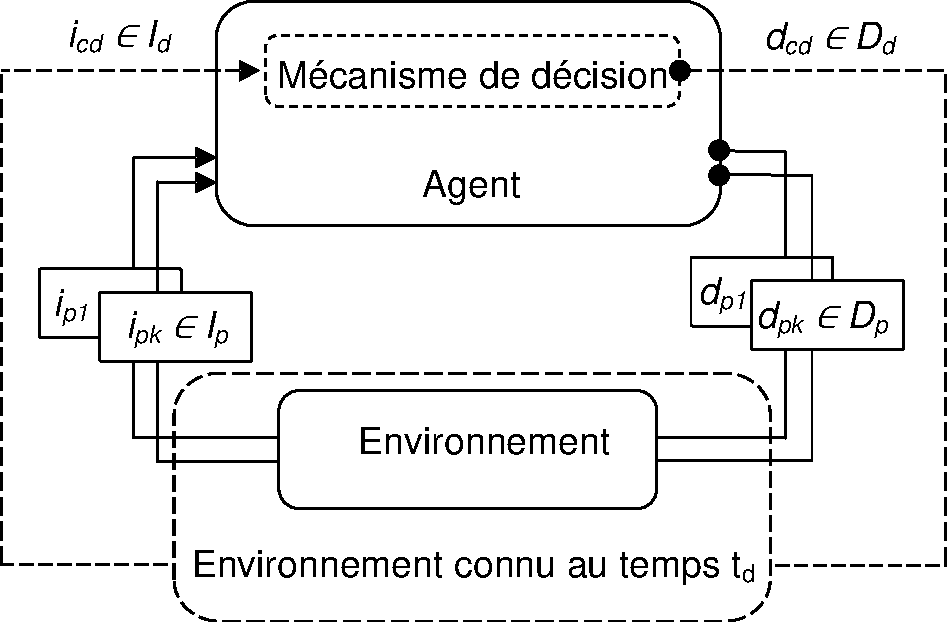
\includegraphics[width=0.4\textwidth]{Figures/4_ir.pdf}
	\caption{Abstraction du cycle EDP, adapté de \cite[Fig.~2]{georgeon_eca_2013}.
		A chaque temps de décision $t_d$, l'agent sélectionne une décision composite $d_{cd} \in D_d$ le conduisant à prendre une série de $k$ décisions primitives $d_{p1} ... d_{pk} \in D_p$ qui résultent en une série de $k$ interactions primitive énactées.
		Du point de vue du système décisionnel de l'agent, tout se passe comme s'il interagissait avec un \og environnement connu au temps $t_d$ \fg à un niveau d'abstraction supérieur.}
	\label{fig:ir}
\end{figure}





Critique de la discrétisation temporelle

Les mécanismes de schéma sont basées sur des cycles d'interaction qui ne permettre qu'une prise en compte d'une temporalité discrète. 
On peut ce demander si cette limitation n'est pas trop contraignante pour permettre de générer des comportements naturels. 

Un contre argument est qu'on peut se fixer des schémas primitifs arbitrairement cours. 
Il faut cependant garder à l'esprit que le mécanisme de schéma permet de monter dans des échelles de temps de plus en plus longues. 




Critique du réductionnisme

Est ce que la théorie de Piaget est trop réductionniste et parvient elle à capture les fondements de la conscience ? 

C'est, à mon sens, la critique principale de cette approche et je n'ai pas la réponse. 